With the RGA in the beam path, we were able to open and close a shutter in the beam path and see an extinction of the water signal, but a more accurate representation would be from the ions in the trap themselves. We know that the trapped \ce{Be+} ions will reaction with \ce{H2O} to predominately produce \ce{BeOH+}, which we see as a drop in the fluorescence. Figure \ref{fig: shutter_closing} shows fits of the fluorescence decay as a beam from the CBGB is suddenly blocked by our shutter in the beam line. Comparing the fitted reaction rates, we find that they agree with the background rates found as shown in figure \ref{fig: shutter_bkg}. This indicates to us that we indeed have a beam of cryogenic water coming from the CBGB, as seen by the sudden extinction of the \ce{Be+ + H2O} reaction.

To accurately control the reactions occurring in the ion trap, it is ideal to be able to quickly turn the beam on and off. Controlling the fill lines outside of the chamber is not ideal, as thin tubing was used, yielding very low conductances. The characteristic time of flow through a tube can be shown to be $\tau_{\mathrm{tube}} = C V$, where $C$ is the conductance and $V$ is the volume of the tube in question. Turning on and off the flow outside of the chamber would give time constants in the range of seconds. To more deterministically control the beam flux, we insert a vacuum compatible Uniblitz VS35 35mm Optical Shutter in the beam line. The shutter does not create a seal within the chamber, background gasses may flow around and influence the beam.

Running the beam with the shutter in between the RGA and experimental cell, we find that there is a distinct difference in the \ce{H2O} signal when the shutter is open and closed. Using laser cooled \ce{Be+}, we find the difference in the reaction rate both independently, as well as in situ, shown in Figures \ref{fig: shutter_bkg} and \ref{fig: shutter_closing}.

\begin{figure}[H]
	\centering
	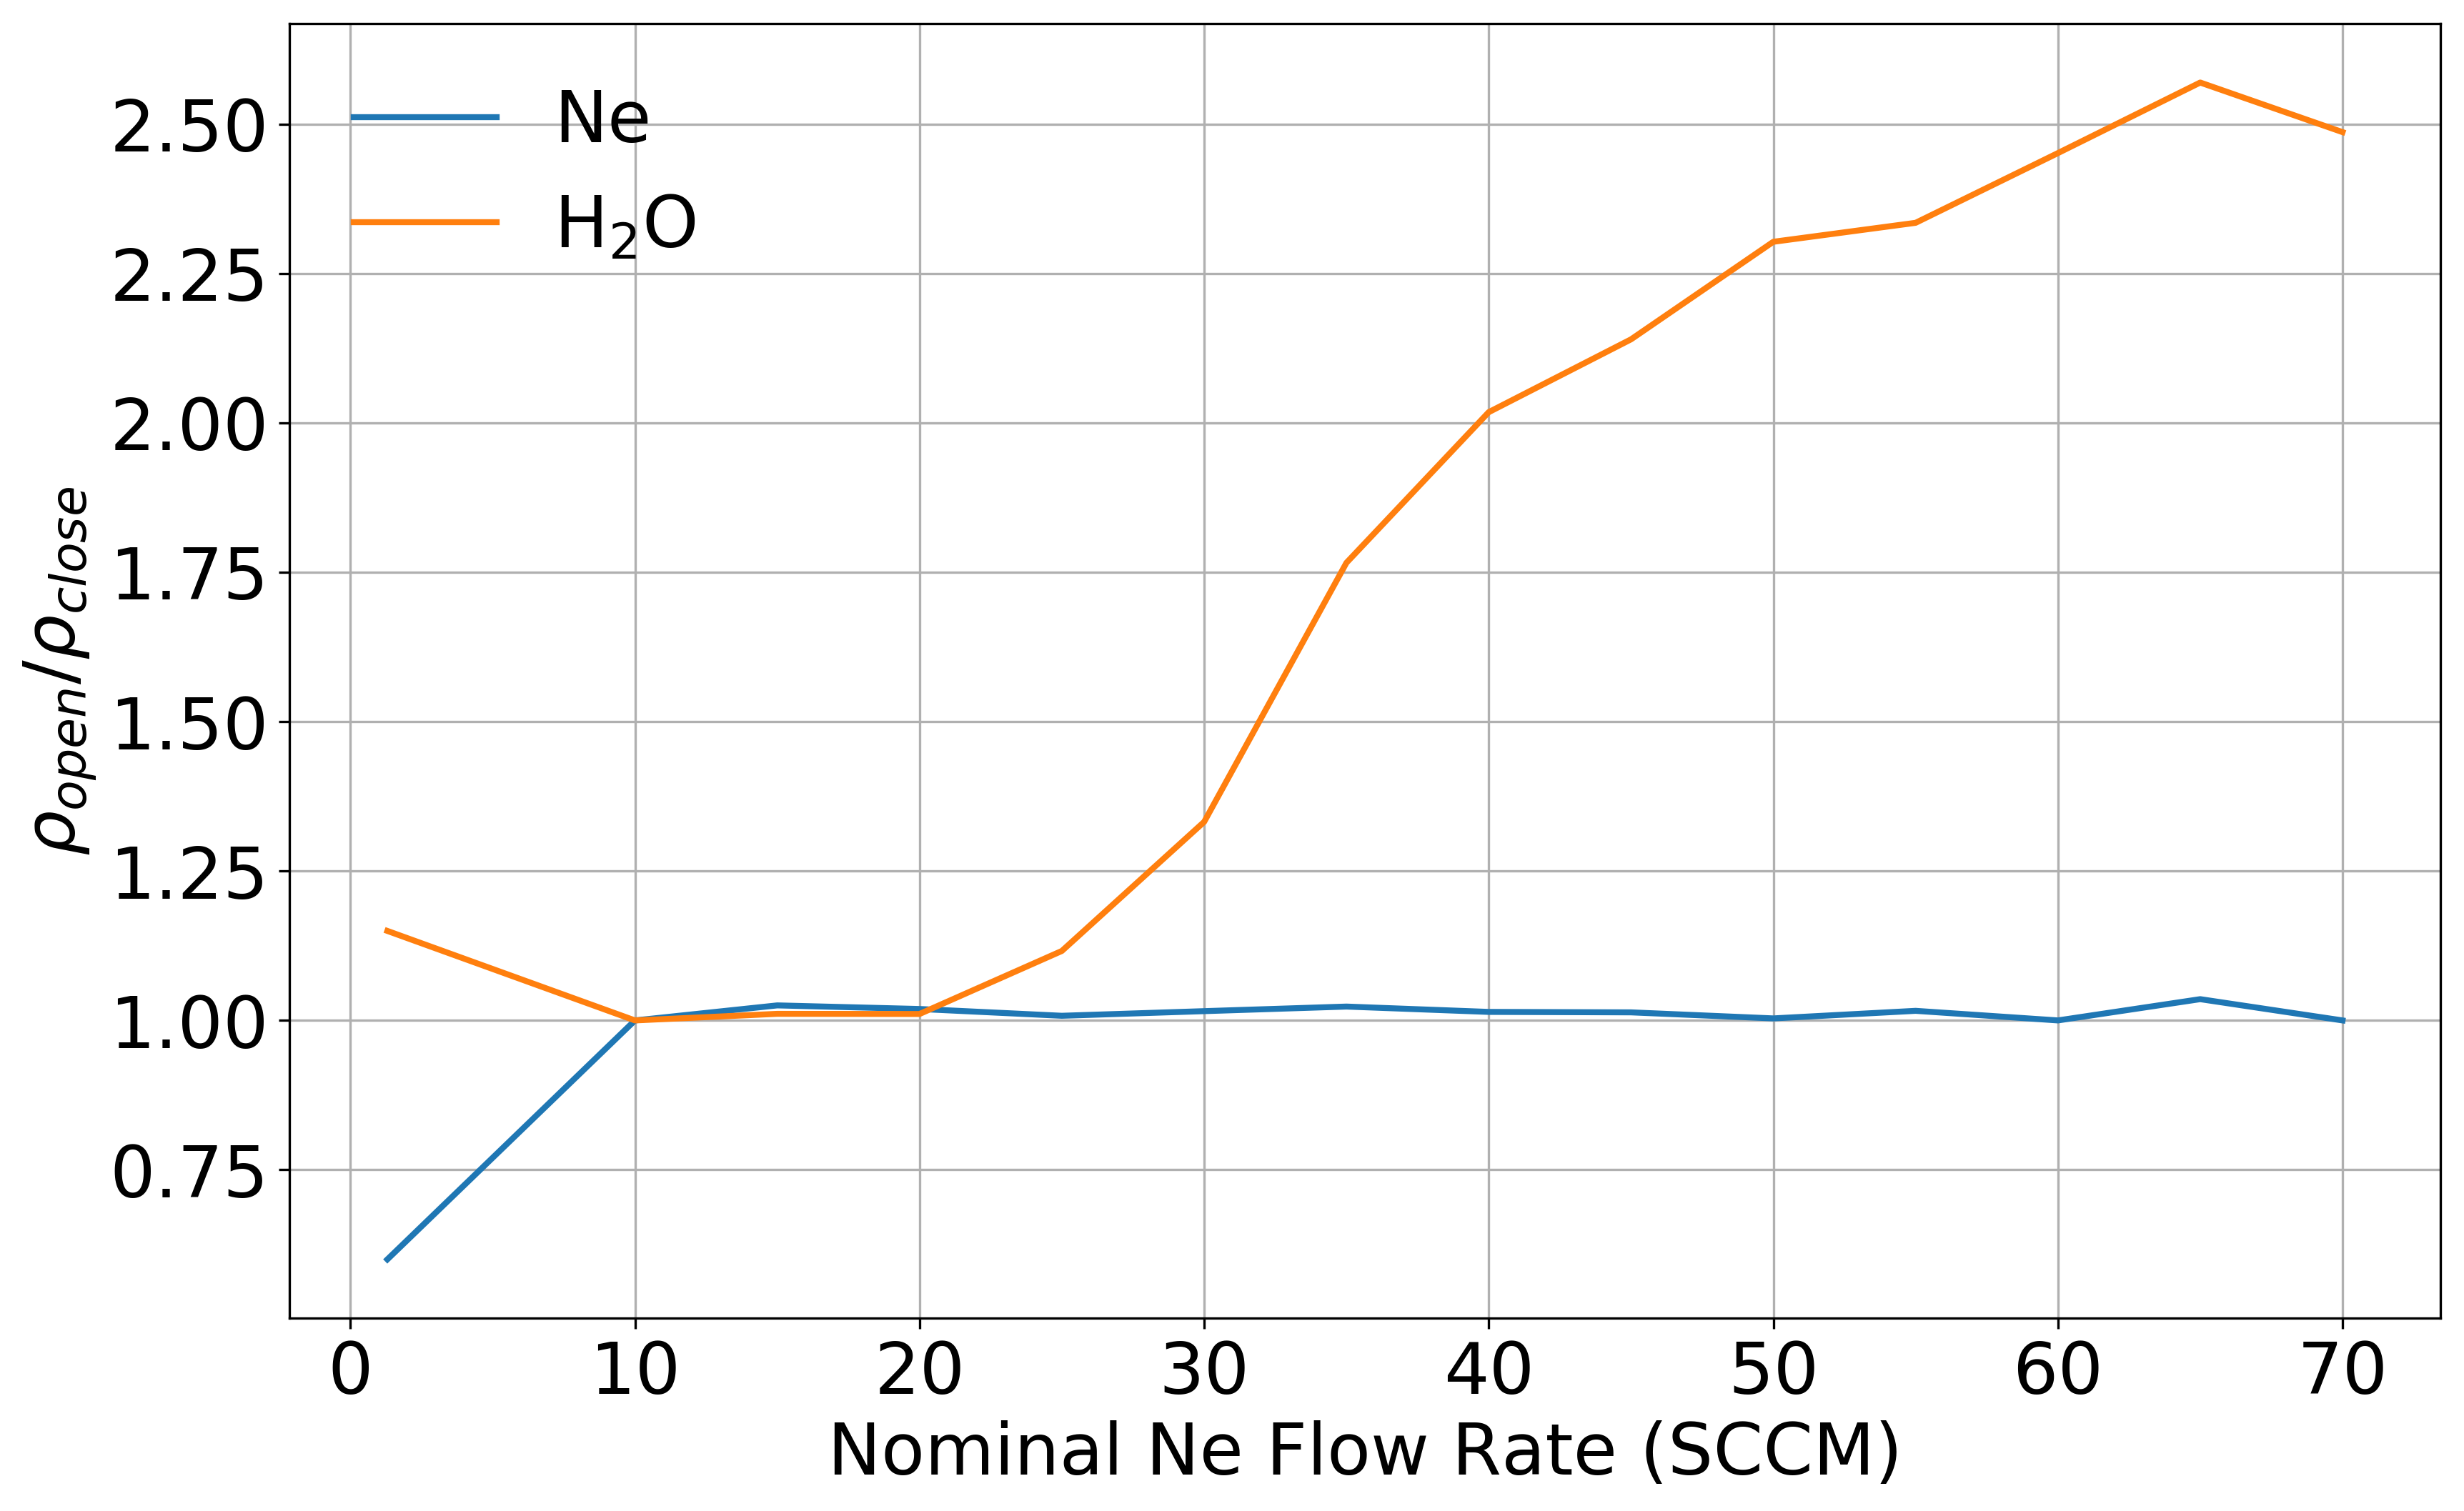
\includegraphics[width=0.8\textwidth]{images/CBGB_RGA_contrast.png}
	\caption{Ratios of water and neon from the beam when the Uniblitz shutter is opened and closed. Detection is done via RGA placed 30 cm from the cell aperture.}
	\label{fig: RGA contrast}
\end{figure}

\begin{figure}[H]
	\centering
	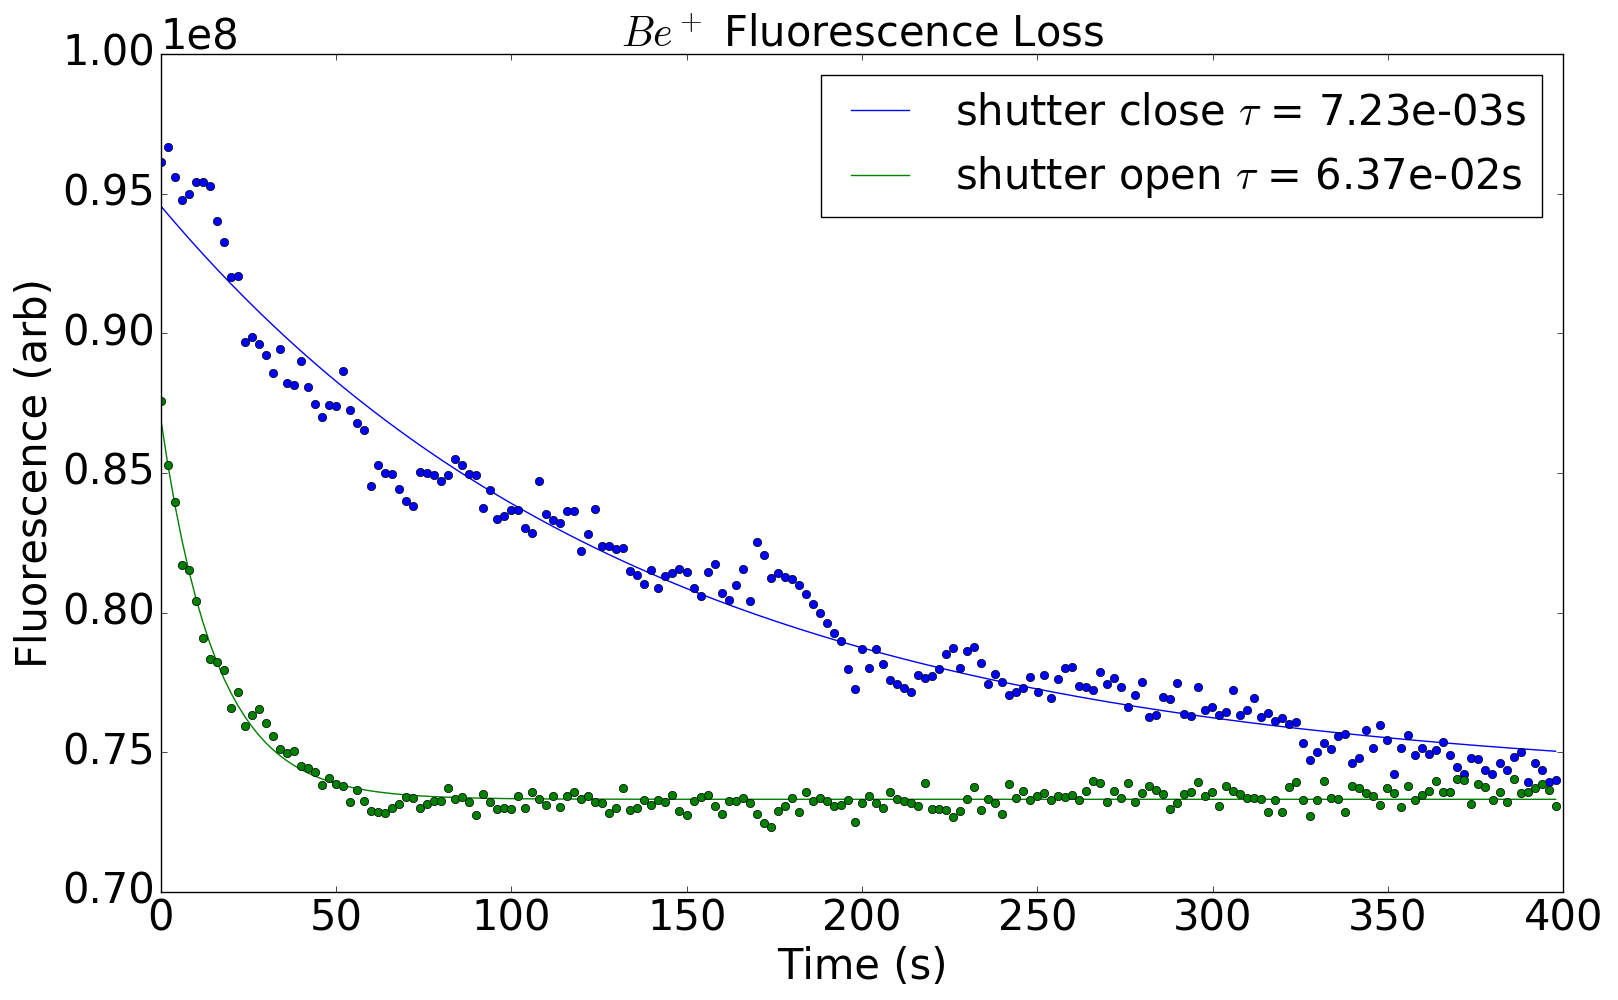
\includegraphics[width=0.8\textwidth]{images/CBGB_sudden_shutter_flow_bkg.png}
	\caption{Fluorescence decays of loaded \ce{Be+} ions exposed to a cold water beam with an inline shutter either opened, in green ($\tau = 7.23 \times 10^{-3}$s) or closed, in blue ($\tau = 6.37 \times 10^{-2}$s)}
	\label{fig: shutter_bkg}
\end{figure}

\begin{figure}[H]
	\centering
	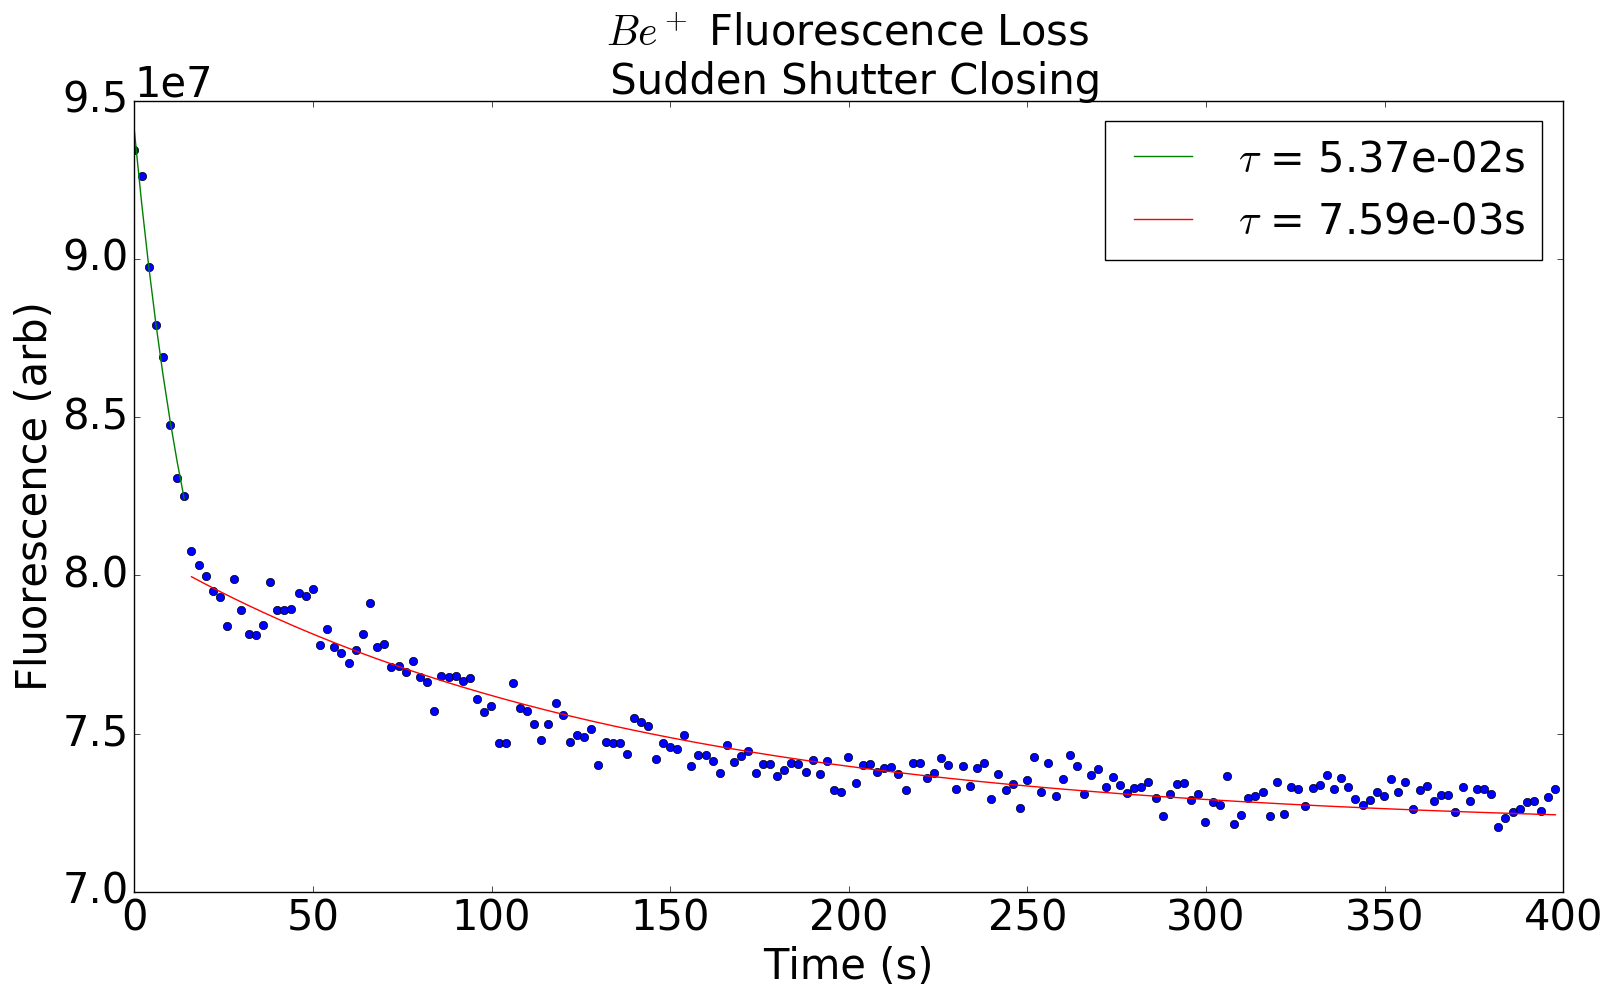
\includegraphics[width=0.8\textwidth]{images/CBGB_sudden_shutter_flow.png}
	\caption{Fluorescence decays of loaded \ce{Be+} ions exposed to a cold water beam with an inline shutter opened, in green ($\tau=5.37 \times 10^{-2}$s) or closed, in red ($\tau=7.59 \times 10^{-3}$s)}
	\label{fig: shutter_closing}
\end{figure}